\section{Theorie}
\label{sec:Theorie}

\subsection{Mikrowellen}
Mikrowellen sind Elektromagnetische Strahlung.
Ihr Spektrum bewegt sich in einer Frequenz von 1 bis 300 \si{\giga\Hz} dies entspricht einem Wellenlängen bereich von etwa \SI{30}{\centi\meter} bis \SI{1}{\milli\meter}.
Der etwas irreführende Name kommt aus der Funktechnik, da dort ein Name für Wellen gesucht wurde, dessen Wellenlänge unter der der UKW Strahlung liegt. 
Heute werden Mikrowelle vor allem bei der Nahrungserwärmung genutzt, da sie dafür geeignet sind die Wassermolekühle zu einer Bewegung anzuregen.
\\\\
Dabei sollte gesagt sein, dass die Wellenlänge von Mikrowelle keine Resonanzschwingung auslöst. 
Sonder die Wasserdipole sich nach dem wechselnden Elektrischen Feld der Welle ausrichten.
Die Dipole sind aber zu träge um sich mit der Schwingungsfrequnz des E-Felds auszurichten. 
Dies führt dazu, dass sie sich langsam hin und her bewegen.
Durch diese Bewegung entsteht ein Widerstand gegen das E-Feld und es wird Wärme Energie frei.
\\\\
In unserem Versuch werden die Mikrowellen mit einem Reflexklystron erzeugt.

\subsection{Reflexklystron}
Ein Schema des Reflexklystron ist in Abbildung \ref{fig:reflex_schema} zu sehen.
Es besteht aus einer Heizkathode, einer Reflektor Anode und einem Hohlraumresonantor zwischen Kathode und Anode.
Wenn nun eine Spannung an die Kathode angelegt wird treten an ihr Elektron aufgrund des Glühelektrischen Effekts aus.
Diese werden durch ein Beschleuningungsgitter in Richtung der Refelktoranode beschleunigt.
Auf dem Weg zum Reflektor laufen die Elektronen durch den Hohlraumresonantor.
An diesen ist eine Wechselspannung angelegt, es ensteht ein oszilierendes Elektrisches Feld.
Wenn nun Elektronen zu früh ankommen, sodass sie parallel zu den Feldkompontenten des Feldes laufen werden sie gebremst.
Elektronen die zu spät ankommen laufen antiparallel zu den Elektrischen Feldkompontenten wodurch diese weiter beschleunigt werden.
Dardurch kommt es zu einem Bunching, dies bedeutet, dass sich die Elektronen in Paketen in Richtung des Refelktors bewegen.
Am Refelktor werden sie durch das negative Potential des Reflektors erst gebremst und dann zurück in Richtung Hohlraumresonantor beschleunigt.
\begin{figure}
    \centering
    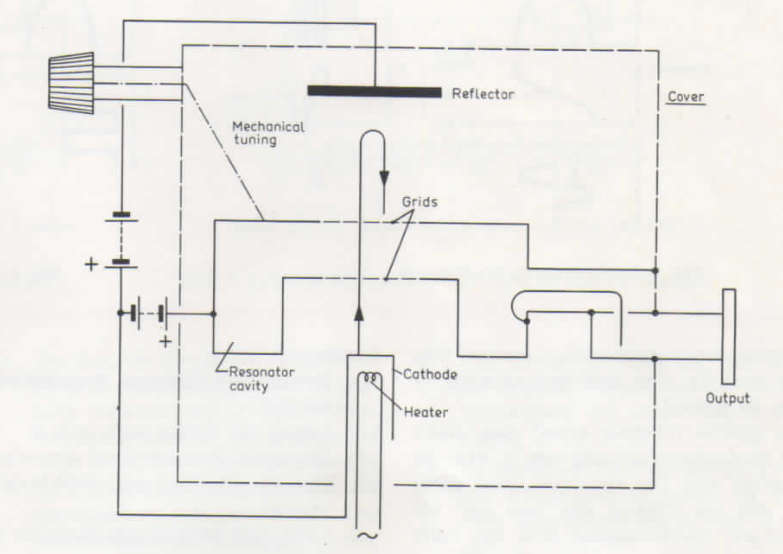
\includegraphics[width=0.75\textwidth]{content/data/reflex_klystron_schema.png}
    \caption{Schema eines Reflexklystron mit mechanischer Abstimmung. Die zwei Pfeile zeigen die Bewegungsrichtung der Elektronen im Refelexklystron an. Bild entnommen aus \cite[6]{Anleitung}}
    \label{fig:reflex_schema}
\end{figure}
\FloatBarrier

Wenn nun die Elektronenpakete wieder in den Resonator eintreten wechselwirken sie mit dem dort vorhandenen E-Feld.
Wenn sie parallel zu den E-Feldkompontenten laufen geben sie Energie an den Resonator ab und verstärken so die Schwigung im Resonator.
Die stärkste Schwingung wir bei einer Verweilzeit von $(n + \frac{3}{4})$ im Resonator erreicht.
Um diesen Punkt zu treffen ist es möglich verschiedene Spannungen am Klystron anzulegen.
Ein Plot zwischen Ausgangleistung und der Refelktorspannung ist in Abbildung \ref{fig:output_refelktor_voltage} zu sehen.
Es ist zu erkennen, dass das Klystron je nach Refelktorspannung in verschiedenen Moden schwingt.
Zudem ist es möglich die Weglänge der Elektronen durch eine mechanische Abstimmung zu verändern.
Diese verändert das Resonatorvolumen.
Eine weiter Methode zur Justage ist die elektronische Abstimmung, was die Änderung der Reflektorspannung und der Resonatorspannung beinhaltet.
In dem hier behandelten Versuch wird die Reflektorspannung rechteck moduliert.

\begin{figure}
    \centering
    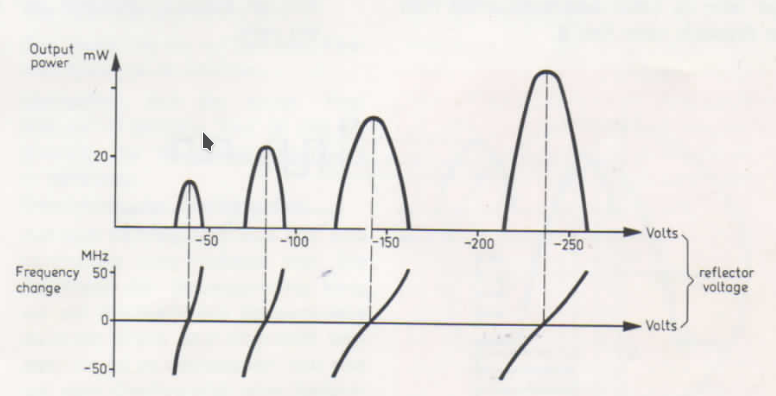
\includegraphics[width=0.75\textwidth]{content/data/refelx_spannung_schema.png}
    \caption{Aufgetragen ist die Output Leistung und Frequenz der Mikrowelle in Abhängigkeit der Reflektorspannung. Bild entnommen aus \cite[6]{Anleitung}}
    \label{fig:output_refelktor_voltage}
\end{figure}

\subsection{Hohlleiter}
Hohlleiter sind im Allgemeinen hohle Metallkörper durch die Energie transportiert wird.
Sie können verschiedene Formen haben und aus unterschiedlichen Metallen bestehen.
In dem behandelten Versuch wird ein rechteckiger Hohlleiter genutzt.
Der Energie Transport findet dabei durch elektromagnetische Wellen statt, die sich durch den Leiter bewegen.
Da der Leiter für die Welle eine räumliche Begrenzung ist können nur Wellen bis zu einer bestimmten Grenzfrequenz
\begin{equation}
    f_\text{c} = \frac{c}{\lambda _\text{c}} \quad \text{mit} \quad \lambda _\text{c} = \frac{2}{\sqrt{ \left ( \frac{m}{a} \right )^2 + \left ( \frac{n}{b} \right )^2}}
    \label{eq:grenzwellenlaenge}
\end{equation}
im Hohleiter propagieren.
Die Grenzwellenlänge $\lambda _\text{c} $wird dabei durch die Moden $m$ und $n$ definiert. Sowie der Ausedehnung des Hohleiters $a, b$.


Die tatsächliche Wellenlänge im Hohlleiter $\lambda _\text{g}$ lässt sich wiederum durch 
\begin{equation}
    \lambda _\text{g} = \frac{\lambda _{0}}{1 - \left ( \frac{\lambda _0}{\lambda _\text{c}} \right )^2}
    \label{eq:wellenlaenge_hohleiter}
\end{equation}
bestimmen.
Wobei $\lambda _0$ die Wellenlänge im freien Raum ist.

E-Wellen schwingen in verschiedenen Moden.
Sie haben eine elektrische Mode und eine magnetische Mode.
In dem genutzen Hohleiter sind die Ausdehnungen so gewählt, das es jeweils nur eine Transversalmode, $TE_\text{m,n}$ und $TM_\text{m,n}$, gibt.
Die beiden Moden wechseln periodisch, nach einer E-Feld Schwingung kommt also immer eine Magnetfeld Schwingung und umgekehrt.
Eine Skizze zu den beiden Moden ist in Abbildung \ref{fig:Moden_Hohleiter} zu sehen.

\begin{figure}
    \centering
    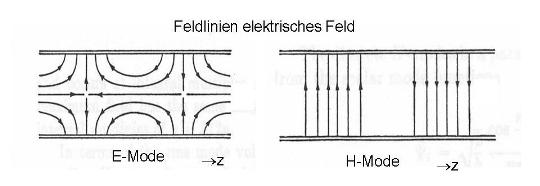
\includegraphics[width=\textwidth]{content/data/Moden_Hohleiter.JPG}
    \caption{Schema der beiden Moden der E-Welle die im Hohleiter auftreten. Bild entnommen aus \cite{wikipedia}.}
    \label{fig:Moden_Hohleiter}
\end{figure}

E-Wellen im Hohleiter können gedämpft werden. Die entsprechende Dämpfung kann durch ein Leistungsverhältnis
\begin{equation}
    \left (\frac{P_1}{P_2} \right )_\text{dB} = 10 \log \frac{P_1}{P_2} = 10 \left ( \log P_1 - \log P_2 \right )
\end{equation}
berechnet werden.

\subsection{Stehwellenverhältnis SWR}
\label{sec:swr}
In einem Hohleiter kann es dazu kommen, dass die erzeugte Welle reflektiert wird und sich diese refelekterte Welle mit der Welle der Quelle überlagert.
So kommt es zu stehenden Wellen die im Allgemeinen störend sind und vermieden werden sollen.
Um die Stärke einer solchen Überlagerung zu messen wird das Stehwellenverhältnis $SWR$ genutzt.
Es ist definiert als 
\begin{equation}
    SWR = \frac{E _\text{max}}{E _\text{min}} = \frac{\left | E _\text{i} \right | + \left | E _\text{r} \right |}{\left | E _\text{i} \right | - \left | E _\text{r} \right |}.
\end{equation}
Das optimale Stehwellenverhältnis wird bei einem Wert von eins erreicht, wobei das schlechteste Stehwellenverhältnis also eine maximale Überlagerung bei $ \infty $ liegt.
Im Versuch wird das beste Stehwellenverhältnis durch einsetzen eines Abschlusses erreicht und die stärkste Reflektierung durch einsetzen eines Kurzschlusses.
Gemessesen wird das Stehwellenverhältnis mit einem SWR-Meter.
Dieses misst das Stehwellenverhältnis in Dezibel oder VSWR wobei die Skalen den Beziehung
\begin{equation*}
    \sqrt{\frac{V_0}{V}}  \quad \text{und}  \quad 10 \, \text{log} \left ( \frac{V_0}{V}\right )  
\end{equation*}
folgen.

